\subsection{Informatik}

\author{Alexander Suter}

\begin{frame}
	\frametitle{Übersicht\hfill{}\footnotesize \group}

	\begin{figure}
		\centering
		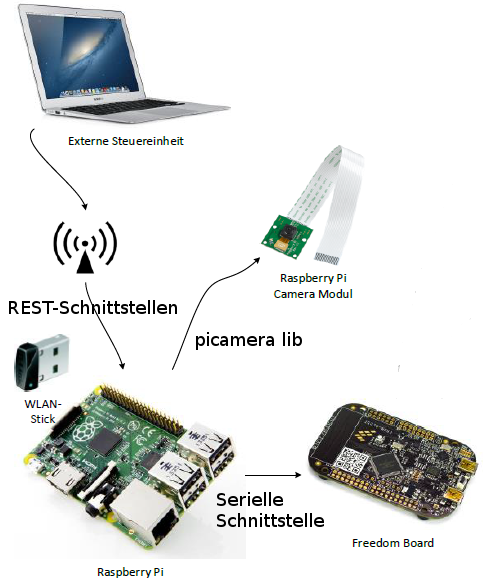
\includegraphics[width=0.5\textwidth]{../../fig/blockdiagramm-informatik.png}
	\end{figure}

\end{frame}

\subsubsection{Bordcomputer}
\begin{frame}
	\frametitle{Bordcomputer\hfill{}\footnotesize \group}
	\framesubtitle{Raspberry Pi}
	
	\begin{figure}
		\centering
		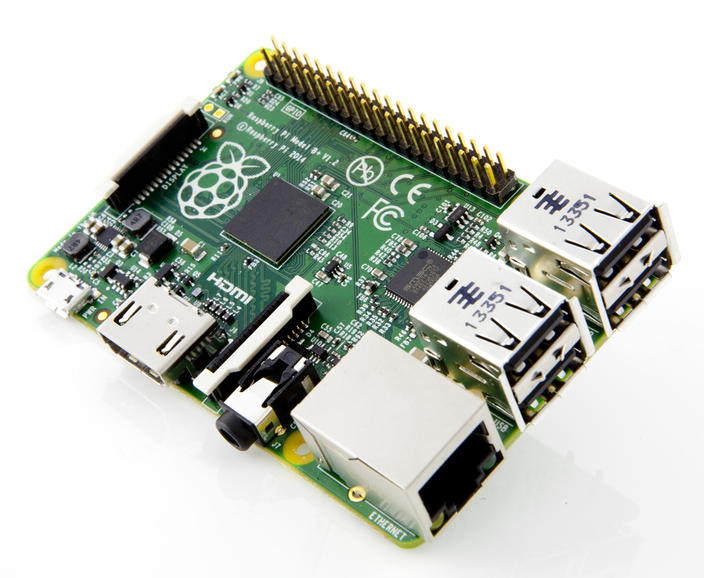
\includegraphics[width=0.6\textwidth]{../../fig/raspberry-pi-b-plus.jpg}
		\caption{Raspberry Pi (B+)}
	\end{figure}
	
    % Warum Raspberry Pi und nicht ein anderes
    % Vorteile des Pi
	
\end{frame}

\subsubsection{Bildverarbeitung}
\begin{frame}
	\frametitle{Bildverarbeitung\hfill{}\footnotesize \group}
	\framesubtitle{Kamera}
	
	\begin{figure}
		\centering
		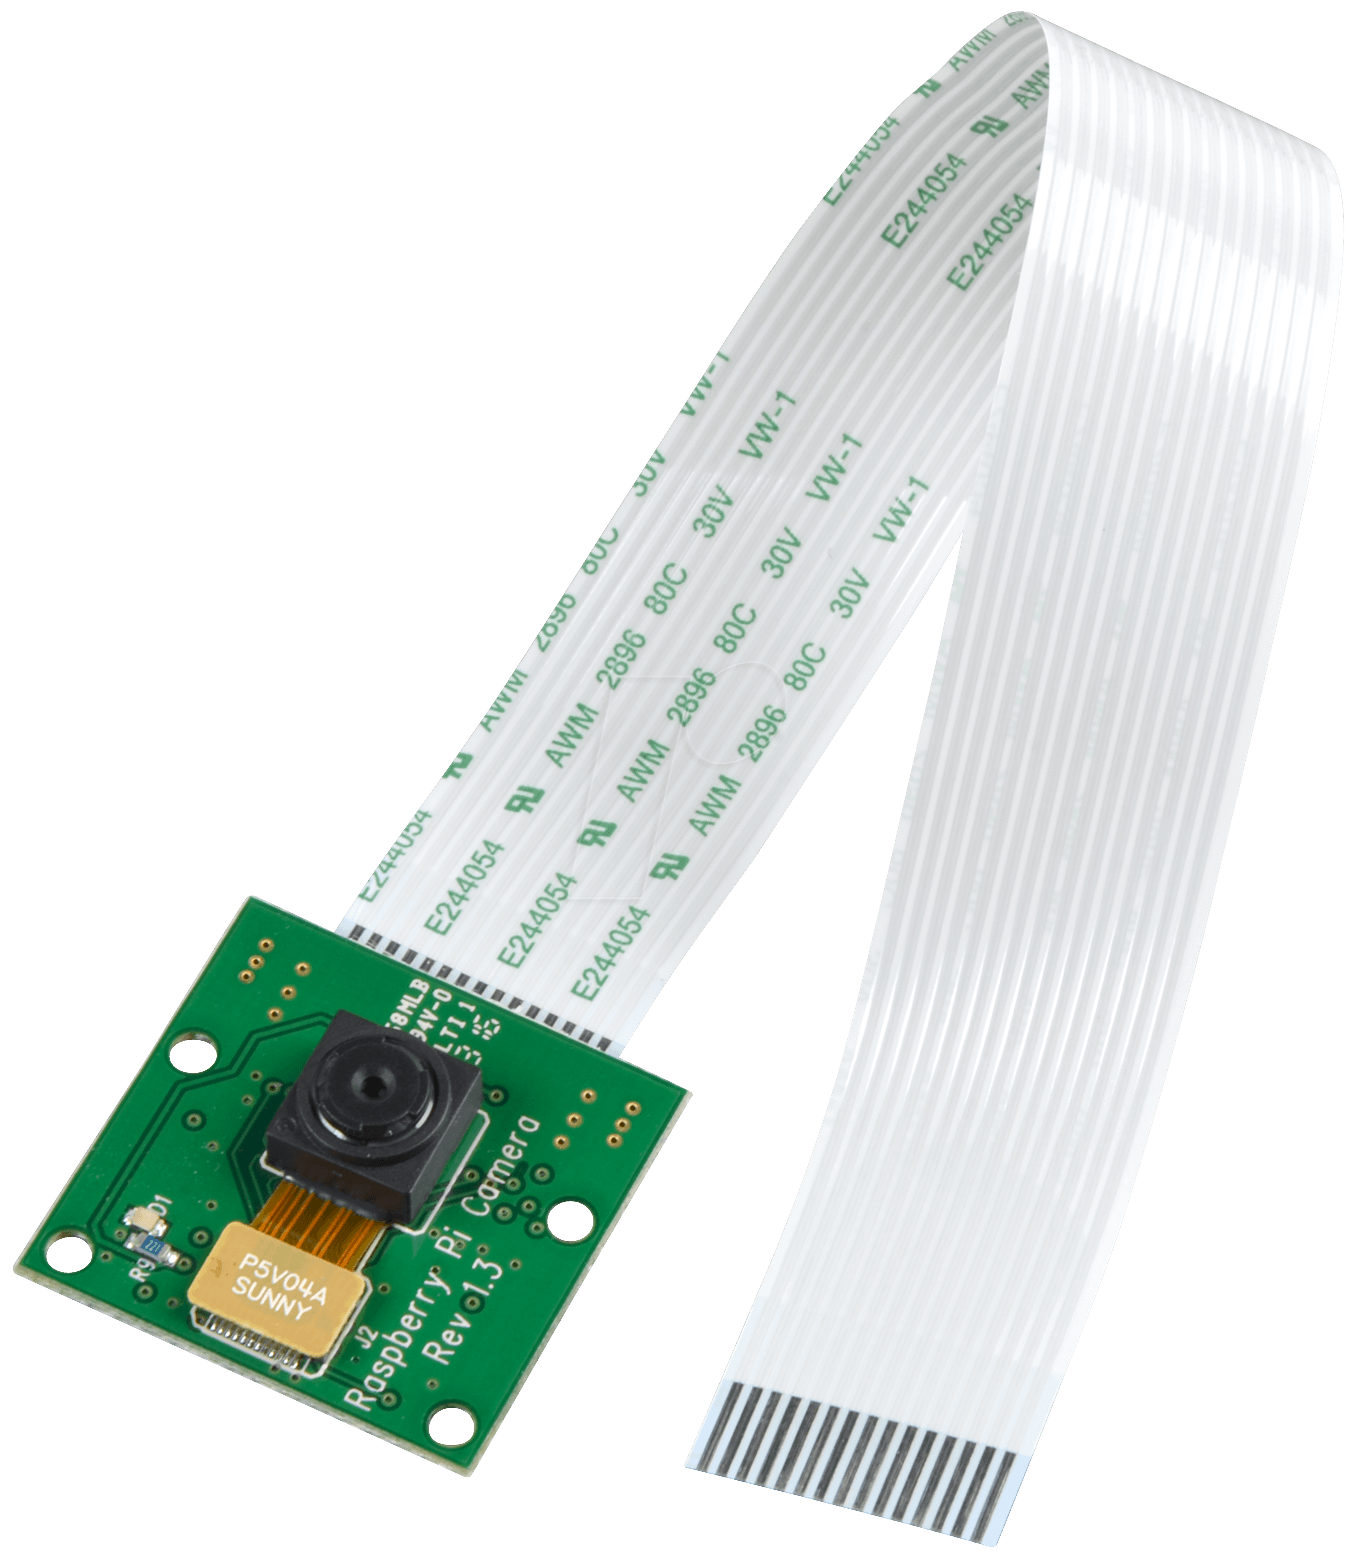
\includegraphics[width=0.4\textwidth]{../../fig/raspberry_pi_cam.png}
		\caption{Raspberry Pi Camera}
	\end{figure}
	
\end{frame}

\begin{frame}
	\frametitle{Bildverarbeitung\hfill{}\footnotesize \group}
	\framesubtitle{Algorithmen zur Informationsauswertung}
	
	\begin{figure}
		\centering
		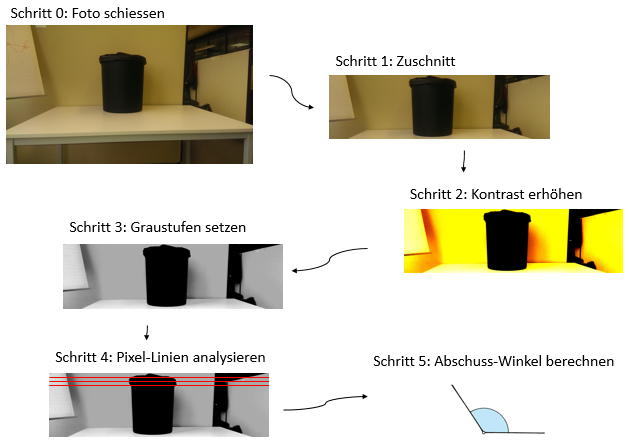
\includegraphics[width=0.8\textwidth]{../../fig/ablauf-ortung-des-korbes-algorithmus.png}
	\end{figure}
	
	% Algorithmus erklären und was die einzelnen
	% Schritte auch technisch machen.
	% Zudem noch die Helligkeit und der Weissablgeich
	% ansprechen.
	
\end{frame}

\begin{frame}
	\frametitle{Bildverarbeitung\hfill{}\footnotesize \group}
	\framesubtitle{Parametrierung des Algorithmus}
	
	\begin{figure}
		\centering
		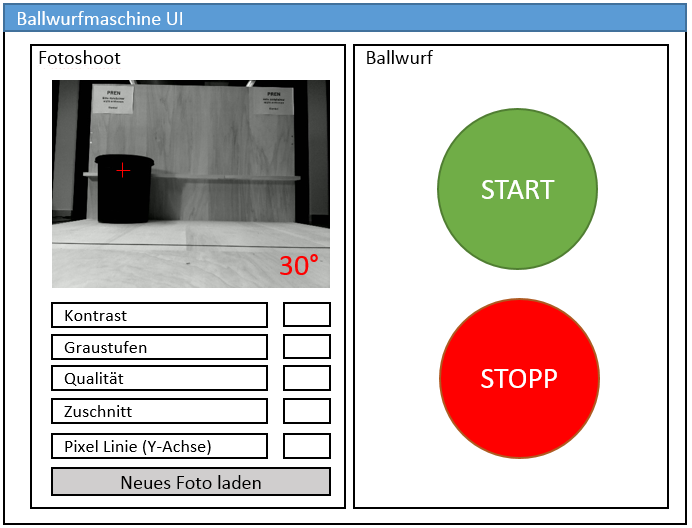
\includegraphics[width=0.6\textwidth]{../../fig/fotoshoot-configurator.png}
		\caption{Ballwurfmaschine UI}
	\end{figure}
	
\end{frame}
